%!TEX root = planning.tex
\section{Function Points: size estimation}
\subsection{Overview} % (fold)
\label{sub:fp_overview}

The \textbf{Function Point approach} is a very useful tool for estimating the effort needed in designing and coding a project. Several aspects are considered for the estimation, as prescribed by the specifications: 
\begin{description}
    \item \textbf{Internal Logic Files}: homogeneous set of data handled by the application being developed;
    \item \textbf{External Interface Files}: homogeneous set of data managed by the application but created elsewhere;
    \item \textbf{External Input}: operation invoked for doing a simple operation on the system with external data (for example, user registration, booking a cab\ldots);
    \item \textbf{External Inquiry}: operation that involves both input and output, mainly for retrieving information from the system;
    \item \textbf{External Output}: system operation producing data for the external environment.
\end{description}

\begin{figure}
\centering
\subfigure[FP Counting Weights]{\label{fig:fp_counting}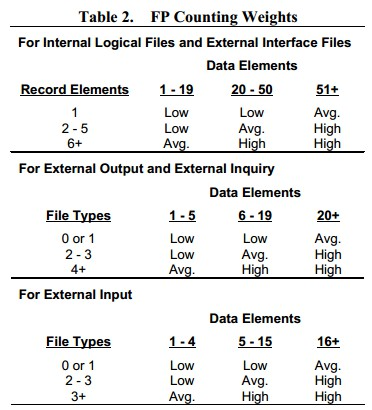
\includegraphics[width=60mm]{img/fpcounting.jpg}}
\subfigure[UFP Complexity Weights]{\label{fig:fp_total}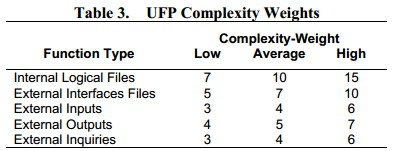
\includegraphics[width=60mm]{img/fptotal.jpg}}
\caption{FP Analysis}
\end{figure}

For each point a \textbf{counting weight} (\emph{Low}, \emph{Avg.} or \emph{High}) has been given according to the parameters specified in Figure~\ref{fig:fp_counting}. After that, a certain amount of FPs has been calculated for each section according to Figure~\ref{fig:fp_total}.

Finally, starting from the total amount of FP, we estimated the project size in SLOC (for more on this, see Section~\ref{sub:results}).

\subsection{Internal Logic Files} % (fold)
\label{sub:ilf}
The application must handle information about the following entities:

\begin{table}[h]
    \label{tab:ilf}
    \centering
    \resizebox{1\textwidth}{!}{
    \begin{tabular}{p{5cm}|cccc}
    \hline

    \hline
    \textbf{File} & \textbf{Record Elements} & \textbf{Data Elements} & \textbf{Counting Weight} & \textbf{FPs} \\
    \hline
        Customer   &   6+     &   51+     &   High    &   15 \\
        Ride       &   6+     &   51+     &   High    &   15 \\
        Call       &   6+     &   51+     &   High    &   15 \\
        TaxiDriver &   6+     &   51+     &   High    &   15 \\
        Address    &   2--5     &   51+     &   High    &   15 \\
        Zone       &   2--5     &   1--19     &   Low    &   7 \\
    \hline
        \textbf{TOT}    &   &   &   & \textbf{82} \\
    \hline
        
    \end{tabular}}
\end{table}

\subsection{External Interface File} % (fold)
\label{sub:eif}
The application must store these information from the external environment:

\begin{table}[h]
    \label{tab:eif}
    \centering
    \resizebox{1\textwidth}{!}{
    \begin{tabular}{p{5cm}|cccc}
    \hline

    \hline
    \textbf{File} & \textbf{Record Elements} & \textbf{Data Elements} & \textbf{Counting Weight} & \textbf{FPs} \\
    \hline
        Maps    &   6+     &   51+     &   High    &   10 \\
        %PaymentInfo    &   2--5    &   51+     &   High    &   10 \\
    \hline
        \textbf{TOT}    &   &   &   & \textbf{10} \\ 
    \hline
        
    \end{tabular}}
\end{table}


\subsection{External Input} % (fold)
\label{sub:ei}
The application must guarantee the following operations for the external environment:

\begin{table}[h]
    \label{tab:ei}
    \centering
    \resizebox{1\textwidth}{!}{
    \begin{tabular}{p{5cm}|cccc}
    \hline

    \hline
    \textbf{Operation} & \textbf{Entities involved} & \textbf{Data Elements} & \textbf{Counting Weight} & \textbf{FPs} \\
    \hline
        Login/signup/logout    &   1     &   16+     &   Avg    &   $3 \times 4$ \\
        Edit/delete profile    &   1     &   16+     &   Avg    &   $2 \times 4$ \\
        Add/delete request/res   &   3   &   16+     &   High    &   $3 \times 6$ \\
        Add/remove/update ride           &    1    &    16+  &  Avg & $3 \times 4$ \\
        Set   taxi status                      &     1    &   16+ &   Avg &   4 \\
        
    \hline
       \textbf{TOT}    &   &   &   & \textbf{54} \\
    \hline
        
    \end{tabular}}
\end{table}

\subsection{External Inquiry} % (fold)
\label{sub:eiq}
The application must make these inquiries available:

\begin{table}[h]
    \label{tab:eiq}
    \centering
    \resizebox{1.1\textwidth}{!}{
    \begin{tabular}{p{5cm}|cccc}
    \hline

    \hline
    \textbf{Operation} & \textbf{Entities involved} & \textbf{Data Elements} & \textbf{Counting Weight} & \textbf{FPs} \\
    \hline
        Get   previous rides    &   2     &   20+     &   High    &   6 \\
        Show  call for a user                &   3      &  20+       & High  & 6 \\
        Check existence of a ride           &   1       &   20+     & Avg   & 4 \\
        Get   info for a ride                 &   1       &   20+     & Avg   &   4 \\  
        Get   pre-calculated fee              &   1       &   20+     &   Avg &   4  \\
    \hline
       \textbf{TOT}    &   &   &   & \textbf{24}\\
    \hline
        
    \end{tabular}}
\end{table}

\subsection{External Output} % (fold)
\label{sub:eo}
The application produces data to the external environment through the following operations:

\begin{table}[h]
    \label{tab:eo}
    \centering
    \resizebox{1.1\textwidth}{!}{
    \begin{tabular}{p{5cm}|cccc}
    \hline

    \hline
    \textbf{Operation} & \textbf{Entities involved} & \textbf{Data Elements} & \textbf{Counting Weight} & \textbf{FPs} \\
    \hline
        Notification to drivers (accepting/refusing ride)              &   2 (Ride \& Customer)       &   20+     &   High &   7  \\
        Notification to customers (ride accepted)           &   2 (Ride \& Taxi)            &   20+     &   High    & 7 \\
        Confirmation email (after signup)             &       1                           &   20+     &   Avg     & 5 \\
    \hline
       \textbf{TOT}    &   &   &   & \textbf{19} \\
    \hline
        
    \end{tabular}}
\end{table}

\subsection{Results} % (fold)
\label{sub:results}
% >>>>>>>> TODO: così siamo a 189, mi sembra veramente tanto. DA RIVEDERE
According to \cite{bib:fp}, the following holds for J2EE:
\begin{equation}
    \frac{\mbox{SLOC}}{\mbox{FPs}} = 46
\end{equation}

If we sum all the results we got from the previous sections and multiply it by 46, we get ??? lines of code.
% DIRE quanto giusto / sbagliato sia questo numero di SLOC